\chapter{Experiments}%
\label{ch:experiments}

\section{Datasets}
In this section we introduce the two datasets we will be working on. First a simplified Toy dataset which reduces the problem to a minimla canonical one and second the musdb18 dataset which is a widely-used testset for musical source separation.

\subsection{ToyData}
\begin{marginfigure}[5em]
    \resizebox{\textwidth}{!}{%
        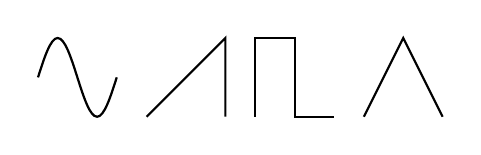
\begin{tikzpicture}
    \node[matrix,thick,column sep=1em,row sep=1em]
    {
        \draw (0,0.5) sin (0.25,1) cos (0.5,0.5) sin (0.75,0) cos (1,0.5); &
        \draw (0,0) -- (1,1) -- (1,0); &
        \draw (0,0) -- (0,1) -- (0.5,1) -- (0.5,0) -- (1,0); &
        \draw (0,0) -- (0.5,1) -- (1,0); \\
    };
\end{tikzpicture}
%
    }%
    \caption{One period of each of the four toy sources: sinus, sawtooth, square and triangle wave.}%
    \label{fig:toy_data}
\end{marginfigure}

We simplify the problem domain to create a toy-like dataset. We randomly generate waves from four simple oscillations, see~\cref{fig:toy_data}. Given a wave from each source, the mix is computed by simply taking the mean. When sampling from each source we randomly select a period and phase. The frequencies are restricted to the frequency bounds of the 88 keys of a equal-temperament tuned piano. In our experiments we are gonna model these sources with probability densities, looking especially at the square that will pose a problem, as those only consist of two unique values (\(-1\) and \(1\)). This collapsing posterior would simplify the problem too much, therefore we also vary the amplitude of the sampled signals in the uniform range \([0.8, 1.0]\).

In ++later++ section we show that estimating densities over these waves is not giving a smooth manifold. Or differently: in the latent space we can not interpolate between two signals, because the model models, simply put, the sample waves as spiked Dirac deltas.


\subsection{musdb18}
Further we use the \emph{musdb18}~\cite{rafiiMUSDB182017} dataset published for the 2018 Signal Separation Evaluation Campaign~\cite{stoter20182018}. The datasets consists of 150 full songs covering various artists and genres, splited into train and test sets sized 100 and 50, respectively. Each track is separated into the four sources \emph{drums}, \emph{bass}, \emph{vocals} and \emph{others}. The \emph{others} source channel contains any set of instrument not categorized under the first three ones. The song files are provided in the Stem audio file format~\cite{nativeinstrumentsStem} and encoded at 44.1kHz. Stem here is terming the provided source channels, we use the terms interchangeably.

Next to the separated stems, the dataset provides the original (studio) mix for each song. This mix is not equivalent to the simple linear mixing which we get by taking the mean. Nevertheless the provided mix diverges only insignificantly from a auto-generated mix, as the original sources are provided in their post-compression, post-mixed form. This means that we can use the original mix and assume it to be reasonably close to the canonical linear mix.

As the songs are real natural songs, they are of different lengths. Our models will, in difference to many other recent methods, not be auto-regressive. Thus we sample fixed-length cuts from the songs as training and test samples. For the musdb data no pre-processing is applied, as the data already contains the wanted level variability, it spanning different genres and artists.

It is noted that the musdb18 dataset, while providing a remarkable diverse 10hr of real-world music, is a rather small numbered set of samples. Any data modeling from this set of data will consequently be biased. The dataset specifically is created for the accompanying separation challenge and will not translate to general music modeling.

For both the Toy Data and the musdb18 dataset we experiment with prior models on time-domain and spectral-domain input.

\section{Testing the priors}

\subsection{Adding noise}
\begin{marginfigure}
    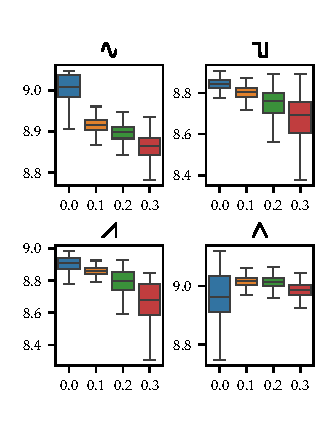
\includegraphics{noise_likelihood_with_noise}%
    \caption{noise likelihood with noise}%
    \label{fig:noise_ll_with_noise}
\end{marginfigure}

In this ablation study we want to check how resilient the generative prior models are to noisy samples. It is hypothesized that the latent space of the model consists of, intuitively, singular peaks at mappings of in-distribution samples~\cite{jayaramSource2020}. For the separation to be able to optimize under the prior density, we need likelihood to slowly decrease when moving away from positive samples. If the distribution is too peaked only noiseless inputs would be highly likely and adding noise quickly makes samples too unlikely. We propose adding Gaussian noise with a random variance to the positive samples during training. This should smooth out the modeled density.

\begin{marginfigure}
    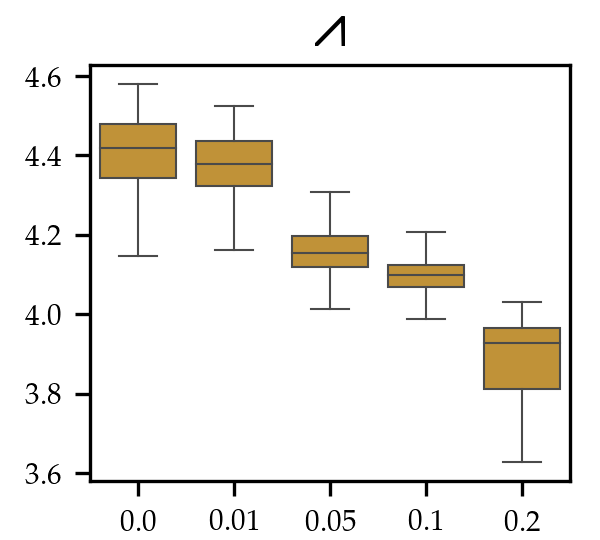
\includegraphics{noise_likelihood_without_noise}%
    \caption{noise likelihood without noise}%
    \label{fig:noise_ll_without_noise}
\end{marginfigure}

\subsection{Testing cross-likelihood}
In the full model each prior is used to extract its source channel separately. Through their training they explicitly contract the density for the positive, in-class examples. During separation the priors therefore encounter negative, out-of-distribution samples for the first time. To be useful for separation, it is important that the priors give a low likelihood to samples from the other classes of the dataset.

\begin{marginfigure}
    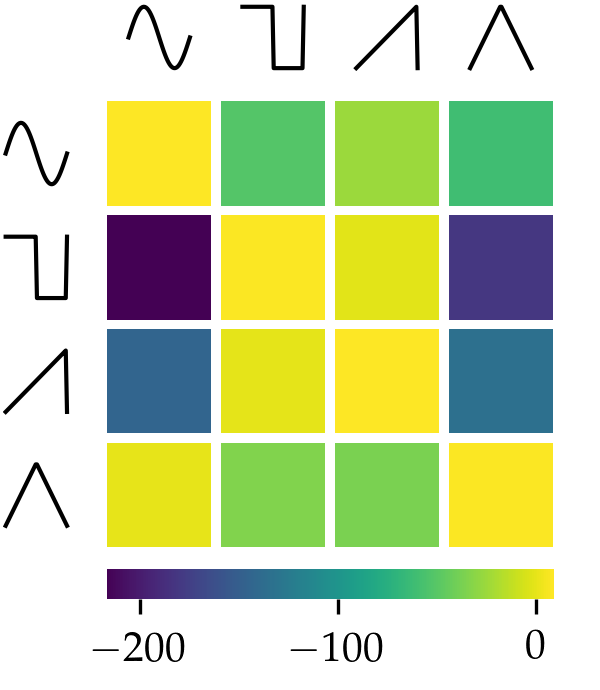
\includegraphics{heatmap_toy}%
    \caption{We display the mean average log likelihood of the test data under the different priors and the different signal sources.}%
    \label{fig:heatmap_toy}
\end{marginfigure}

We test for this by calculating the mean log likelihood of the the test data set under each prior, for each source channel separately. What we anticipate is that the samples from the priors training source are of high likelihood while all other sources are low likelihood. In \cref{fig:heatmap_toy} we show the source dependent likelihoods for the Toy Data. The in-distribution samples are all of high likelihood while all out-of distribution samples are highly un-likely. The Flow model therefore was able to detect out-of-distribution samples while only being trained on in-distribution samples~\footnote{Something psychological research has shown, humans being able to do.}. The estimated densities are discriminative.

When running the same experiment for the musdb18 the discriminative power does not hold up, see~\cref{fig:heatmap_musdb}. All signal sources are about equally likely under each prior density. We hypothesize this stems from the fact that the real musical data is severely more complicated compared to the Toy Data. The Flows model the appearance of sound in general, as the in-class variability of sounds is already high, without knowing anything about the \I{discriminative} differences between the instruments and does not infer the distribution from those features.

\begin{marginfigure}
    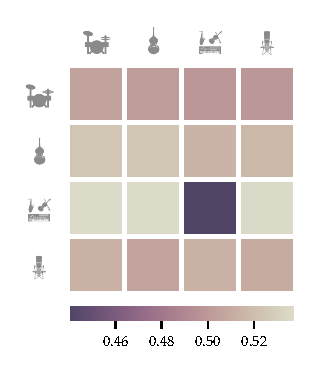
\includegraphics{heatmap_musdb}%
    \caption{We display the mean average likelihood of the test data under the different priors and the different signal sources.}%
    \label{fig:heatmap_musdb}
\end{marginfigure}

Even above that the results exhibit an additional failing for the musdb18 dataset. The third stem in the dataset files \I{other} is filled with a smorgasbord of different instruments. With our training regime we are implying we can model the sound this set of unrelated instruments with only in-distribution samples with a resulting distribution which is discriminative against another set of unrelated instruments. Intuitively this already fails to be reasonable. Because of this the results show the unintuitive result that the test samples from the \I{other} class are \I{less likely} under its own prior model compared to the out-of-distribution samples. While this makes it rather final that the at hand dataset is not completely suitable to out trainings regime, it is a data-dependent restriction that would not correspond to our hypothesized application.

Similar results were shown before in~\itodo{cite some OOD VAE stuff}.

The results for both datasets are similar for all tested model architectures and input domains. See Appendix~\itodo{add results} for the full results.

\subsection{Increasing discriminative power}
With the prior models being not discriminative, it is not possible to train the separation model. Following we will try extend the priors to increase their discriminative power. Above that we propose that our method still holds merit given these results, further work on generative models might result in more discriminative generative models. The method can use any density as a drop-in replacement for the prior in the separation model.

As layed out in~\ref{ch:background} the bad out-of-distribution detection of generative models is not a surprising result and multiple recent works go about solving this. We want to increase the

\begin{marginfigure}
    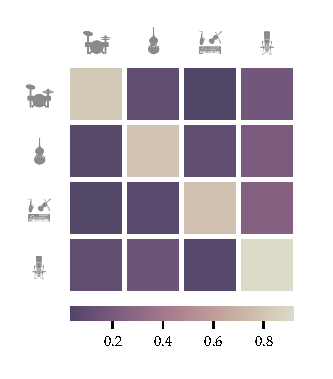
\includegraphics{heatmap_musdb_classifier}
    \caption{The logits of different classes of the different outputs}%
    \label{fig:heatmap_musdb_classifier}
\end{marginfigure}

\section{Testing the posteriors}
\subsection{Denoising autoencoder}

\subsection{TODO EXPERIMENTS}
\begin{enumerate}
    \item Adding noise ⇒ better likelihood
    \item De-noising single signals
\end{enumerate}
